\chapter{Diabetes}

%%%%%%%%%%%%%%%%%%%%%%%%%%%%%%%%%%%%%%%%%%%%%%%%%%%%%%%%%%%%%%%%%%%%%%%%%%%%%%%%%%%%%%%%%%%%%%%%%%%%%%%%%%%%%%%%%%%%        CHAPTER 0   : A long term disorder                %%%%%%%%%%%%%%%%%%%%%%%%%%%%%%%%%%%%%%%%%%%%%%%%%%%%%%%%%%%%%%%%%%%%%%%%%%%%%%%%%%%%%%%%%%%%%%%%%%%%%%%%%%%%%%%%%%%%%%%%%%%%%%%%%%%%%%%%%%%%%%%%%%%%%%%%%%%%%%%%%%%%%%%%%%%%%%%%%%%%%%%%%%%%%%%%%%%%%%%%%%%%%%%%%%%%%%%%%%%%%%%%%%%%%%%%%%%%%%%%%%%%%%%%%%%%%%%%%%%%%%%%%%%%%%%%%%
\section{A long term disorder}%"Biological side"%}
Diabetes occurs when the body stops producing insulin, usually without any early-warning sign in the case of type 1 diabetes. The young patient is often admitted in the hospital with a very high level of sugar in blood, suffering from what is called hyperglycemia.
\paragraph{}

% #ref Type 1 diabetes, novo nordisk%
We assume that "diabetes" stands for "type 1 diabetes" in the following section. Nothing can be done to prevent the onset of diabetes, and research still doesn't know why the disease occur. Diabetes develops when the immune system starts destroying the cells of the pancreas involved in the creation of insulin. The immune system normally protects the body by destroying foreign substances such as bacteria. 

\subsection{Food and insulin}
Glucose is an essential fuel for the organism, used by the organs such as muscles or the brain. Glucose comes from food and is released in the blood during digestion. Blood glucose regulation is done by two hormons: insulin and glucagon. No matter the individual had an important meal a couple of hours before or fasted all the day, blood glucose is always between 4 and 7 mmol/l. 
\paragraph{Insulin and glucagon.} After a meal, blood glucose is high. Insulin is then released, making the blood level decrease till it reaches a normal level, while the extra glucose is stored in the liver and the organs. When the level of glucose becomes too low, glucagon is produced, and some glucose contained in the liver is release in the blood. 

\subsection{Two insulins, two key functions}
%#ref nice graph p.20 of https://shop.diabetes.org.uk/usr/downloads/Carbs-Count-2012-reduced.pdf, can be used%
Insulin as an hypoglycemic hormon, which means that it makes blood glucose decrease. 
%Insulin is a hormone which is produced by the beta cells in the pancreas. Insulin acts like a key to unlock cells. It allows glucose in the blood stream to enter the cells. When insulin is not present, glucose cannot enter the cells and it builds up in the blood. %
Basal insulin and bolus insulin are the two types used for diabetes treatment. Bolus insulin is injected after each meal in order to compensate the amount of glucose absorbed by eating. It's a short acting insulin. However, a minimal amount of insulin is needed all day long because organs need a little insulin to be able to break glucose into energy. For this purpose, basal insulin is injected once a day, it's the long acting insulin. 

%However, insulin plays another key role: making the glucose usable by the organs. %
\subsection{Symptoms}
High blood glucose is called hyperglycemia, and is due to a lack of insulin. Thus, muscles cannot turn blood glucose into energy to use it, given that insulin is needed for this process. An important hyperglycemia is caracterized by an extreme tiredness and a very high blood glucose. The body react trying to get rid of some glucose by the urins. Patient will need to drink large amounts of water and urinate unusually often. 

Low blood glucose is called hypoglycemia, and occurs mainly because of too much insulin injected. The patient may feel dizzy, tired and can loose consciousness. Sugar need to be eaten quickly in order to rise blood glucose to a normal level.  

\subsection{Treatment}
Daily insulin injections are the only way to treat diabetes. Patients need to learn how to inject, and how much insulin they inject. Carbohydrate counting allow them to match their insulin requirements with the amount of carbohydrate they eat and drink. 
\paragraph{Carbohydrate is a nutrient} When broken-down into glucose, it is used as energy by the body. We can classify them in two main types: starchy carbohydrates and sugars.
Starchy carbohydrates comes from pasta, bread, rice and potatoes. Sugars designate table sugar, fructose (found in fruits) and lactose (found in dairy foods). Some foods and drinks do not contain any carbohydrate at all.
%#ref, Carbs count, published by Diabetes UK © 2011 %

Bolus insulin is usually taken around meal time. To find how much bolus insulin is needed, patients should know:
1. How much insulin is needed for a certain amount of carbohydrates. This ratio is individual to each person, and tend to increase during adolescence.
2. The amount of carbohydrates they will eat and drink for this meal.

%Nice example in page 30 of the book%
For instance, if a patient has:
\begin{itemize}
\item A ratio of 1:10, 1 unit of insulin for 10 grams of carbohydrates
\item A lunch with 60g of carbohydrate
\end{itemize}

He will then inject 6 units of insulin to meet his needs. 
\\A correction dose of insulin can be added, for example if the patient didn't take enough insulin before the previous meal or had some snack between. Most people will need 1 unit of bolus insulin to reduce blood glucose levels by 2–3 mmol/l %#reference, mandatory, from https://shop.diabetes.org.uk/usr/downloads/Carbs-Count-2012-reduced.pdf%.
\paragraph{Working out the amount of carb in a meal}
There are various way to figure out the amount of carbohydrates available in a given food, among which we can cite:
\begin{itemize}
\item Reading food labels
\item Using reference lists, provided in the book given by the hospital, in some applications, or in tables such as in figure~\ref{fig:table}
\end{itemize}

\subsection{Long term effects and complications}
The high and low blood glucose a patient can be corrected as descibed above, but being used to a poor blood glucose regulation has also long term effects. Blood vessels are damaged, increasing the risk of heart diseases. Two other organs are the first affected: eyes and feet. Sight loss and foot ulcers are more likely to occur if you have diabetes.  
%%%%%%%%%%%%%%%%%%%%%%%%%%%%%%%%%%%%%%%%%%%%%%%%%%%%%%%%%%%%%%%%%%%%%%%%%%%%%%%%%%%%%%%%%%%%%%%%%%%%%%%%%%%%%%%%%%%%        CHAPTER 0   : Introduction                %%%%%%%%%%%%%%%%%%%%%%%%%%%%%%%%%%%%%%%%%%%%%%%%%%%%%%%%%%%%%%%%%%%%%%%%%%%%%%%%%%%%%%%%%%%%%%%%%%%%%%%%%%%%%%%%%%%%%%%%%%%%%%%%%%%%%%%%%%%%%%%%%%%%%%%%%%%%%%%%%%%%%%%%%%%%%%%%%%%%%%%%%%%%%%%%%%%%%%%%%%%%%%%%%%%%%%%%%%%%%%%%%%%%%%%%%%%%%%%%%%%%%%%%%%%%%%%%%%%%%%%%%%%%%%%%%%
\section{Enhancing diabetes management/"Psycological issues"}

Diabetes Psychology problems
Diabetic adolescents
Motivation to help them 

%%%%%%%%%%%%%%%%%%%%%%%%%%%%%%%%%%%%%%%%%%%%%%%%%%%%%%%%%%%%%%%%%%%%%%%%%%%%%%%%%%%%%%%%%%%%%%%%%%%%%%%%%%%%%%%%%%%%        CHAPTER 0   : Patient education                %%%%%%%%%%%%%%%%%%%%%%%%%%%%%%%%%%%%%%%%%%%%%%%%%%%%%%%%%%%%%%%%%%%%%%%%%%%%%%%%%%%%%%%%%%%%%%%%%%%%%%%%%%%%%%%%%%%%%%%%%%%%%%%%%%%%%%%%%%%%%%%%%%%%%%%%%%%%%%%%%%%%%%%%%%%%%%%%%%%%%%%%%%%%%%%%%%%%%%%%%%%%%%%%%%%%%%%%%%%%%%%%%%%%%%%%%%%%%%%%%%%%%%%%%%%%%%%%%%%%%%%%%%%%%%%%%%
\section{Patient education}
This Msc project is led by the University of Manchester and the Royal Manchester Children’s Hospital. 
\\When a child is first diagnosed, he is admitted in the hospital for a couple of days, usually 3 to 6 days. Medical care is provided in the very beginning and during his stay according to his condition. At the same time, the diabetes team, including doctors, nurses and dieteticians are meeting him regularly. This section will mainly focus on the issue of patient education at the hospital, including "the newly diagnosed sessions" and the "".
\\
\subsection{In the literature}
\subsection{Experience on the ward}
In order to get a better understanding of patient's experience and expectations, I went to the hospital to attend the educational sessions. I was taught as if I was a real patient, and invited to ask the questions a teenager could ask. Trying to react as a 'normal' patient was a way to collect the amount of knowledge they have, and the approach that is used to teach them.
\\In Royal Manchester Children’s Hospital, there is 4 sessions, 2 with the diabetes nurse, and 2 with the dietetician. It may be underestimating to say that patients are often upset while they attend these sessions because they learnt only one or two days before that they were suffering from diabetes, a long term disorder.

%%%%%%%%%%%%%%%%%%%%%%%%%%%%%%%%%%%%%%%%%%%%%%%%%%%%%%%%%%%%%%%%%%%%
\subsubsection{Sessions with the nurse}
\paragraph{Deroulement}
\paragraph{More about patient}
\paragraph{Content to be used by the software}
Motivations to do well: 
-wee when is hyper
-not nice when hypo, looks silly

\subsubsection{Sessions with the dietetician}
\paragraph{The activities of the session}
Presentations usually follow the same pattern. 
\begin{itemize}
\item The dietetician begins with general advices in healthy eating
\item Carbohydrates awareness is raised by the use of the "eatwell plate", representing a healthy balanced diet as shown in picture~\ref{fig:eat_wp}.
\item Carbohydrate counting is explained
\item Explains how to make use of the diffent kinds of sugar %classified by 'speed'% 
and talks about the glycemic index
\item The snacking issue is adressed
\item Activities and small exercices are given to make sure the patients understood the different issues
\end{itemize}
 
 
\begin{figure}
  \caption{The eatwell plate}
  \centering
  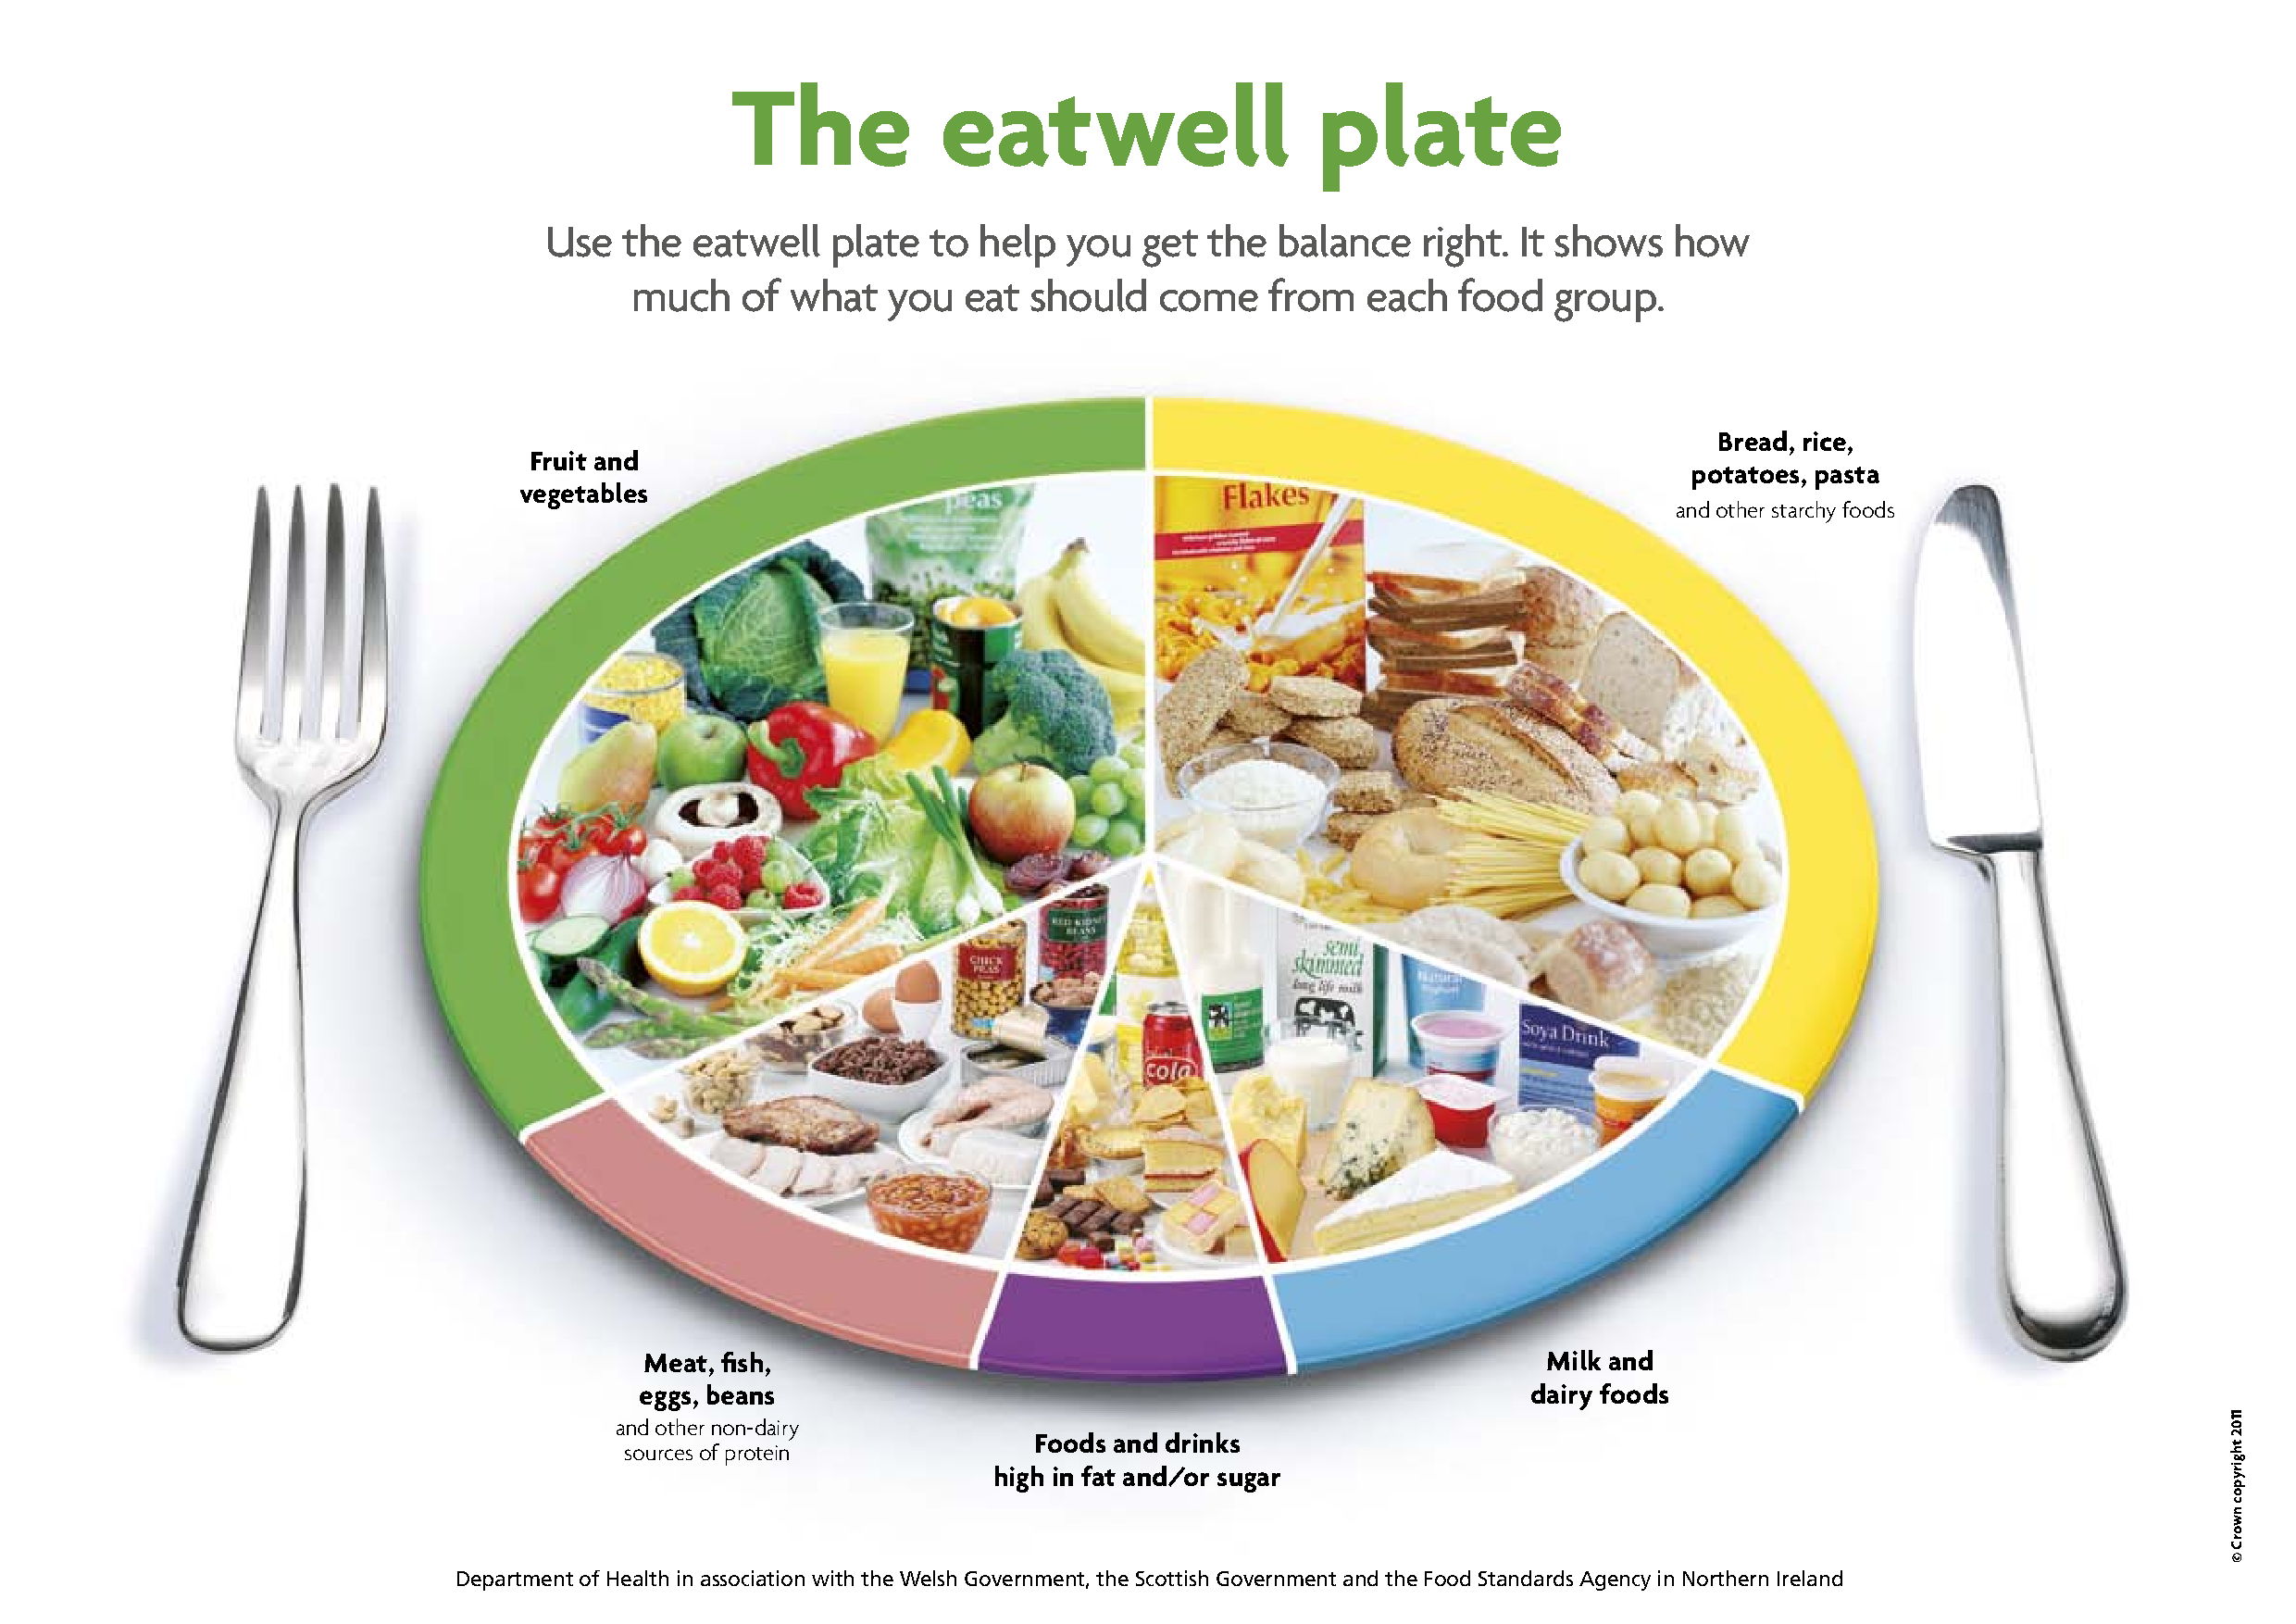
\includegraphics[scale=0.43]{theeatwellplate.pdf}
  \label{fig:eat_wp}
\end{figure}


\paragraph{Patient - Practician %Health professional%
relationship}
Like with the nurse, the patient is quite unwell and tend not to be engaged %careful, mindful% 
during the explanations. It's even harder because they are usualy quite familiar with dietetic advices - they have been treaten at school already - and because non following the advices won't have the same direct effects a forgotten injection can have. The dietetician tries to teach patients according to their specificities. She often cares about:
\begin{itemize}
\item The age or the ability of the patient affects carbohydrate counting, as it needs some basic mathematic skills like the cross product. When they are to young to do this, parents attend to counting carbohydrates for each meal. Being as brief as possible during the explanations allows the practician to focus on key points. For example, emphasing on non-skipping insulin injections instead of explaining exactly why the same amount of insulin cannot be taken for the same kind and quantity of food for two different lunches.
\item 
\item 
\item 
\end{itemize}

The dietetician keeps in mind that some patients are
-young, cannot compute
-not necessary to go through all details: ex of the effects of fat
-try to detect some possible inconsistency as patients tend to present the facts slightely differently: about snacking
-adapted to the status: explain 
-some patients tend to stop eating carbs to avoid insulin injections
\paragraph{Content to be used by the software}
Carbohydrate counting explained. Tips. List of common misconceptions. Multiple Choice Questions (MCQ) and exercices. 
\paragraph{Carbohydrate counting}

\section{Available tools}
